% !Mode:: "TeX:UTF-8:Hard"
\documentclass[a4paper,11pt,twoside]{book}
%\documentclass[paper=8.5in:11in,pagesize=pdftex]{book}
%\usepackage{CJKutf8}
\usepackage[T1]{fontenc}
\usepackage{pifont}
\usepackage{graphicx}
\usepackage{multirow}
\usepackage{longtable}
\usepackage{capt-of}
\usepackage{color}  
%\usepackage[paperwidth=8.5in, paperheight=11in]{geometry}
\usepackage[margin=1.1in]{geometry}
%\usepackage[pass]{geometry}

\newcommand{\linuxcommand}[1]{\texttt{\textcolor{blue}{\$ #1 \Pisymbol{psy}{191}}}}
\newcommand{\op}[1]{\textcolor{blue}{-#1}}
\newcommand{\hotkey}[1]{\framebox{#1}}
\newenvironment{screen}{\sffamily}{\rmfamily}

% for C/C++ frame box
\usepackage{listings}
%\definecolor{mygray}{rgb}{0.9,0.9,0.9}

\lstset{ 
  %backgroundcolor=\color{mygray}, basicstyle=\footnotesize
  mathescape=true,
  frame=single,
  language=c++,
  basicstyle=\footnotesize,
  %literate={\ \ }{{\ }}1
  tabsize=2,
  framextopmargin=0.5em,
  framexbottommargin=0.5em,
  morecomment=[s][\color{red}]{/*-}{*/},
}

\newcommand{\Hilight}[1]{\makebox[0pt][l]{\color{yellow}\rule[-3pt]{#1em}{11pt}}}
\newcommand{\HilightLine}[2][yellow]{\makebox[0pt][l]{\color{#1}\rule[-4pt]{#2em}{13.9pt}}}
%\newcommand{\tophline}{\hline }
%\newcommand{\bottomhline}{\\ \hline }

%\newcommand{\Hilight}[1]{}
%\newcommand{\HilightLine}[2][yellow]{}
\newcommand{\tophline}{ }
\newcommand{\bottomhline}{ }


\newcommand{\specialcell}[2][c]{%
  \begin{tabular}[#1]{@{}l@{}}#2\end{tabular}}

%\addtolength{\oddsidemargin}{-.375in}
%	\addtolength{\evensidemargin}{-.375in}
%	\addtolength{\textwidth}{1.25in}

%	\addtolength{\topmargin}{-.375in}
%	\addtolength{\textheight}{1.75in} 



\begin{document}
%\begin{CJK*}{UTF8}{song}
\title{Drops of knowledge of C++}
\author{Yan Zhao}
\date{}\maketitle

\setcounter{secnumdepth}{4}
\setcounter{tocdepth}{4}
\tableofcontents


\chapter{Basic Syntactic}

\section{Basic C/C++ Contents}
\subsection{basic definition}
\begin{itemize}

\item gogo 
	
\begin{tabular}{|c|c|c|}

	\textbf{type} & \textbf{read} & \textbf{write} \\

	primitive (char, int, float) & pass value & pointer or reference \\

	class, array, structure  & const pointer or reference &  pointer or reference  
\end{tabular}
\item gogo \newline

\begin{tabular}{|c|c|c|}
	
	go go go go go go go let let let let let letgo go go go go go go let let let let let let &  go go go go go go go let let let let let letgo go go go go go go let let let let let let&
	go go go go go go go let let let let let letgo go go go go go go let let let let let let  \\
	
	primitive (char, int, float) & pass value & pointer or reference \\
	
	class, array, structure  & const pointer or reference &  pointer or reference  
\end{tabular}

\item gogo 

\begin{tabular}{|p{0.3\textwidth}|p{0.3\textwidth}|p{0.3\textwidth}|}
	\tophline
	go go go go go go go let let let let let letgo go go go go go go let let let let let let &  go go go go go go go let let let let let letgo go go go go go go let let let let let let&
	go go go go go go go let let let let let letgo go go go go go go let let let let let let  
	\\ \tophline
	
	primitive (char, int, float) & pass value & pointer or reference \\ \tophline
	class, array, structure  & const pointer or reference &  pointer or reference \bottomhline
\end{tabular}


    \item C++ is a Multi-paradigm language, there are five paradigms: 
    
    \begin{enumerate}
        \item Procedural programming. (traditional C programming)
        \item Object-base programming. (class and object)
        \item Object-orient programming. (inheritance)
        \item Generic programming. (template)
        \item functional programming
    \end{enumerate}

\begin{figure}[h]
	\centering
	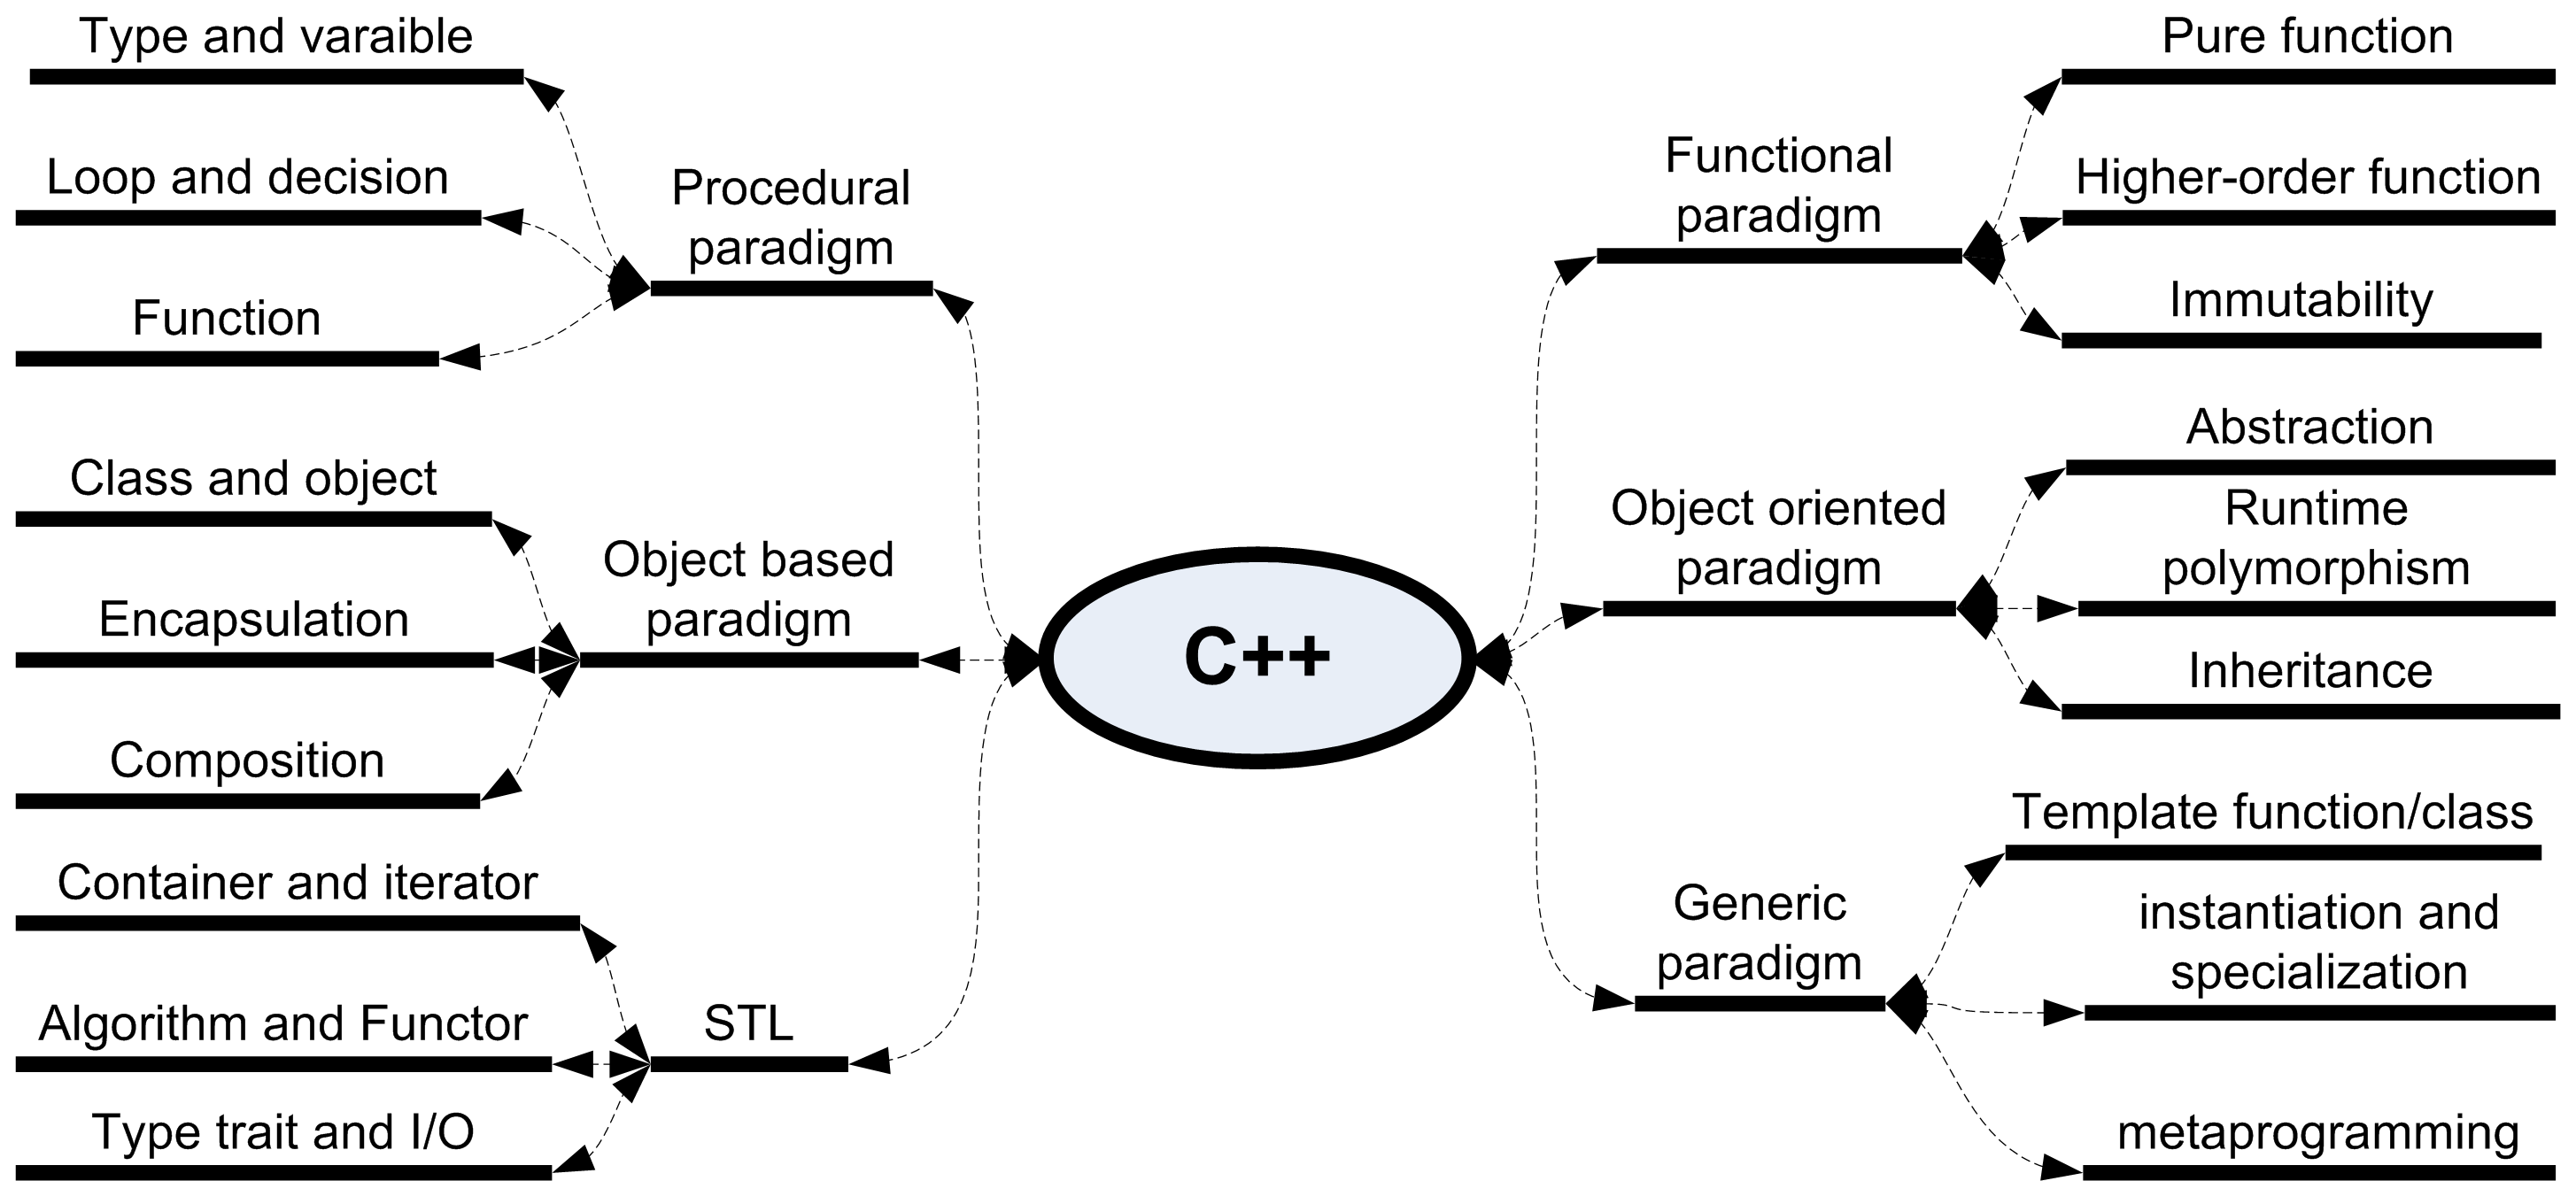
\includegraphics[width=0.85\linewidth]{pics/whole.png}
	\caption{The main component of C++ language}
	\label{fig:whole}
\end{figure}

     \item C++ inherits basic data type, variable name, statement, expression, and operator, control flow, function, file, head file and library, array, pointer and structure from C language. C++ is superset of C, so any C programs can be compiled by C++.
    
    \item Duration and scope are two different conceptions in C++. there are three kinds of duration: \textbf{automatic, static and dynamic.} there are four kinds of scopes:
    \begin{enumerate}
        \item global.
        \item In C++, we can use namespace to add more scopes to divide global scope.
        \item file(translation unit).
        \item local, function local and class local. 
    \end{enumerate}
    
    \item Statement and expression are two important conceptions, you can see their definition in cppreference.com to see academic explanation.
    
    \item Statements are fragments of the C++ program that are executed in sequence. Only statement, which end with semicolon is executed. Most statements are expression statements. 
\begin{lstlisting}[frame=single, language=c++]    
	int n = 1;               // declaration statement
	n = n + 1;               // expression statement
	std::cout << n << '\n'; // expression statement
	return 0;               // return statement
\end{lstlisting}
	\item An expression is a sequence of \textbf{operators} and their \textbf{operands}, that specifies a computation. Expression evaluation may produce a result

    \begin{enumerate}
    	\item Expression: Something which evaluates to a value. Example: \texttt{1+2/x}
    	\item Statement: A line of code which does something. Example: \texttt{GOTO 100;} and statements are all end with semi-comma.
    \end{enumerate}

    \item Function call is a expression, because it can yield a value.
    
    \item \textbf{All expressions yield a value, So expression is a value, statement is an action.}
    

    \item The designers of C realized that no harm was done if you were allowed to evaluate an expression and throw away the result. In C, every syntactic expression can be a made into a statement just by tacking a semicolon along the end:
    
\begin{lstlisting}[frame=single, language=c++]
x+y //is expression;
x+y; //is statement, but you throw away the result
j=i; is a statement.
fun(i) //is expression;
\end{lstlisting}
    
\end{itemize}


\end{document}

